\subsection{Experimental protocol and reporting status}

The final residual GMM-head model follows the same strict split philosophy as the recent
distribution-first models. The split is a city-holdout split with
\texttt{split\_seed = 42}, \texttt{val\_ratio = 0.15}, and
\texttt{test\_ratio = 0.15}. Metrics and losses are computed only on valid
ground pixels, using the target-specific no-data masks and the explicit
LoS/NLoS masks. The model input contains nine spatial channels:

\begin{enumerate}
\item normalized topology,
\item LoS mask,
\item NLoS mask,
\item ground mask,
\item combined path-loss prior,
\item LoS path-loss prior,
\item NLoS path-loss prior,
\item delay-spread prior,
\item angular-spread prior.
\end{enumerate}

The scalar UAV height is not appended as a constant image channel. It is
encoded with a sinusoidal embedding and injected into the network through FiLM
conditioning. The final \texttt{try80\_joint\_huge\_pathloss\_finetune}
configuration uses a shared encoder-decoder with
\texttt{base\_width = 128}, \texttt{cond\_dim = 160}, three GMM
components per task and region, \(\alpha\)-gate bias \(-2\), and fixed
residual caps specified separately for path loss, delay spread and
angular spread.

The final checkpoint reported in Chapter~\ref{chap:results}
uses these frozen path-loss and spread priors as anchors. This
section therefore documents both the frozen-prior inputs and the residual
architecture used by the final evaluation.

\subsection{Prior-Anchored GMM Residual Model}

The final model introduces a joint multi-task residual GMM-head architecture that
predicts a \emph{Gaussian Mixture Model (GMM)} at each pixel, rather than a
simple point estimate. For each task \(k \in \{\mathrm{PL},\, \mathrm{DS},\, \mathrm{AS}\}\),
region \(r\in\{\mathrm{LoS},\mathrm{NLoS}\}\), component
\(j\in\{1,2,3\}\), and valid pixel \(x\), the model predicts a mixture
weight, a mean and a standard deviation. Path loss is modeled in native dB
space, while delay spread and angular spread are modeled in transformed
\(\log(1+y)\) space inside the probabilistic head and converted back to
native units for deterministic metrics.

The native residual caps are task- and region-dependent:

\begin{equation}
\delta_{\max,k,r}
=
\begin{cases}
7~\mathrm{dB}, & k=\mathrm{PL},\ r=\mathrm{LoS},\\
25~\mathrm{dB}, & k=\mathrm{PL},\ r=\mathrm{NLoS},\\
20~\mathrm{ns}, & k=\mathrm{DS},\ r=\mathrm{LoS},\\
20~\mathrm{ns}, & k=\mathrm{DS},\ r=\mathrm{NLoS},\\
17^\circ, & k=\mathrm{AS},\ r=\mathrm{LoS},\\
15^\circ, & k=\mathrm{AS},\ r=\mathrm{NLoS}.
\end{cases}
\label{eq:try80_residual_caps}
\end{equation}

The bounded native residual is assembled from a global map-level offset and a
local pixel-level correction:
\begin{equation}
\Delta_{k,r,j}(x)
=
\mathrm{clip}\!\left(
\delta^{(g)}_{k,r,j}
+
\delta^{(\ell)}_{k,r}(x),
\ -\delta_{\max,k,r},\
\delta_{\max,k,r}
\right).
\label{eq:try80_delta_assembly}
\end{equation}

The mean of each mixture component is then anchored to the frozen prior:
\begin{equation}
\mu^{\mathrm{native}}_{k,r,j}(x)
=
y^{\mathrm{prior}}_{k,r}(x)
+
\alpha_{k,r}(x)\Delta_{k,r,j}(x),
\label{eq:try80_mu}
\end{equation}

where:
\begin{itemize}
\item \(y^{\mathrm{prior}}_{k,r}(x)\) is the frozen regional prior from
      the path-loss or spread prior,
\item \(\delta^{(g)}_{k,r,j}\) is a map-level residual offset for component
      \(j\),
\item \(\delta^{(\ell)}_{k,r}(x)\) is a per-pixel residual refinement shared
      across components,
\item \(\alpha_{k,r}(x) \in (0,1)\) is a learned spatial gate, initialized
      with bias \(-2\), so the model starts close to the prior,
\item the residual is bounded to \(\pm\delta_{\max,k,r}\) to prevent the DNN from
      deviating catastrophically from the prior.
\end{itemize}

For the spread tasks, the native anchored mean is mapped into transformed
space before the Gaussian likelihood:
\begin{equation}
\mu_{k,r,j}(x)
=
\begin{cases}
\mu^{\mathrm{native}}_{k,r,j}(x), & k=\mathrm{PL},\\
\log\!\left(1+\max\{\mu^{\mathrm{native}}_{k,r,j}(x),0\}\right),
& k\in\{\mathrm{DS},\mathrm{AS}\}.
\end{cases}
\label{eq:try80_mu_transform}
\end{equation}

The DNN also predicts per-pixel mixture probabilities \(p_{k,r,j}(x)\) and
component variances:
\begin{equation}
\sigma_{k,r,j}(x)
=
\sqrt{
\left(\sigma^{(g)}_{k,r,j}\right)^2
+
\left(\tilde\sigma^{(\ell)}_{k,r}(x)\right)^2
}.
\label{eq:try80_sigma}
\end{equation}
Both variance terms are constrained by sigmoid transforms to lie between
\(\sigma_{\min}=0.05\) and \(\sigma_{\max}=3.0\). These bounds stabilize the
probabilistic head and prevent the NLL term, when it is enabled, from
collapsing to unrealistically tiny uncertainty or exploding to a uselessly
flat density.

The architecture supports a full GMM Negative Log Likelihood (NLL). The final
\texttt{try80\_joint\_huge\_pathloss\_finetune} checkpoint, however, uses the
same head with an RMSE-dominant fine-tuning objective; its NLL, KL, moment and
outlier-budget weights are set to zero in the resolved YAML configuration. The
deterministic point prediction used for RMSE evaluation is the expected value
of the mixture:

\begin{equation}
\hat z_{k,r}(x)
=
\sum_{j=1}^3 p_{k,r,j}(x)\mu_{k,r,j}(x),
\qquad
\hat y_{k,r}(x)
=
\begin{cases}
\hat z_{k,r}(x), & k=\mathrm{PL},\\
\exp(\hat z_{k,r}(x))-1, & k\in\{\mathrm{DS},\mathrm{AS}\}.
\end{cases}
\label{eq:try80_point}
\end{equation}
The final task map selects \(\hat y_{k,\mathrm{LoS}}\) or
\(\hat y_{k,\mathrm{NLoS}}\) using the explicit CKM LoS/NLoS masks. This
prevents a visually plausible NLoS correction from leaking into pixels whose
geometric path is LoS, and conversely prevents LoS ring structure from being
used as an explanation for blocked pixels.

The training loss also includes a prior-preservation term:

\begin{equation}
\mathcal{L}_{\mathrm{guard},k}
=
\mathbb{E}_{x\in\Omega_k}
\left[
\max\left(0,\,
\left(\hat y_k(x) - y_k(x)\right)^2
-
\left(y^{\mathrm{prior}}_k(x) - y_k(x)\right)^2
\right)
\right]
\label{eq:try80_loss}
\end{equation}

This \emph{pixel-wise} prior guard penalizes the model explicitly on any pixel
where its squared error exceeds the prior's squared error. The guard is not
used alone; it is part of the composite optimization objective in
Sec.~\ref{sec:try80_objective}.

\subsection{Architecture: Shared UNet with FiLM}

The final model processes the map inputs through a shared multi-task
convolutional encoder-decoder. In the final \texttt{huge} configuration,
scalar UAV height is encoded into a condition vector
$\textbf{c} \in \mathbb{R}^{160}$ and injected dynamically into the
convolutional feature maps at multiple scales via
\emph{Feature-wise Linear Modulation (FiLM)} layers.

For a given convolutional feature map $\textbf{X} \in \mathbb{R}^{C \times H \times W}$, a linear projection of the height condition $\textbf{c}$ outputs a scale vector $\textbf{g} \in \mathbb{R}^C$ and a shift vector $\textbf{b} \in \mathbb{R}^C$. The feature map is then modulated via an affine transformation:
\begin{equation}
\textbf{X}' = \textbf{X} \odot (1 + \textbf{g}) + \textbf{b}
\label{eq:film}
\end{equation}
where $\textbf{g}$ and $\textbf{b}$ are broadcasted spatially across the height and width.
The FiLM mechanism and injection points are unchanged between the
\texttt{big} and \texttt{huge} variants; only the width of the feature
maps changes, so the FiLM projection emits \(2C\) parameters for the
larger \texttt{huge} channel counts.

The architecture explicitly enforces the separation of global and local effects via a dual-head design for each task:

\begin{itemize}
\item \textbf{Global Head (Map-Level Context)}: The deepest bottleneck feature map is globally average-pooled to produce a single vector representing the macro-context. This pooled vector, fused with the height condition, is passed through an MLP to predict the non-spatial quantities: mixture probabilities $p_{k,j}$, global offsets $\delta_{\mathrm{global},k,j}$, and global variances $\sigma_{\mathrm{global},k,j}^2$.
\item \textbf{Local Head (Pixel-Level Refinement)}: The high-resolution output of the decoder is passed through $1\times1$ convolutions to predict the spatially varying fields: $\delta_{\mathrm{local},k}(x)$, $\alpha_k(x)$, and $\tilde\sigma_{\mathrm{local},k}^2(x)$.
\end{itemize}

\begin{figure}[H]
\centering
\resizebox{\textwidth}{!}{%
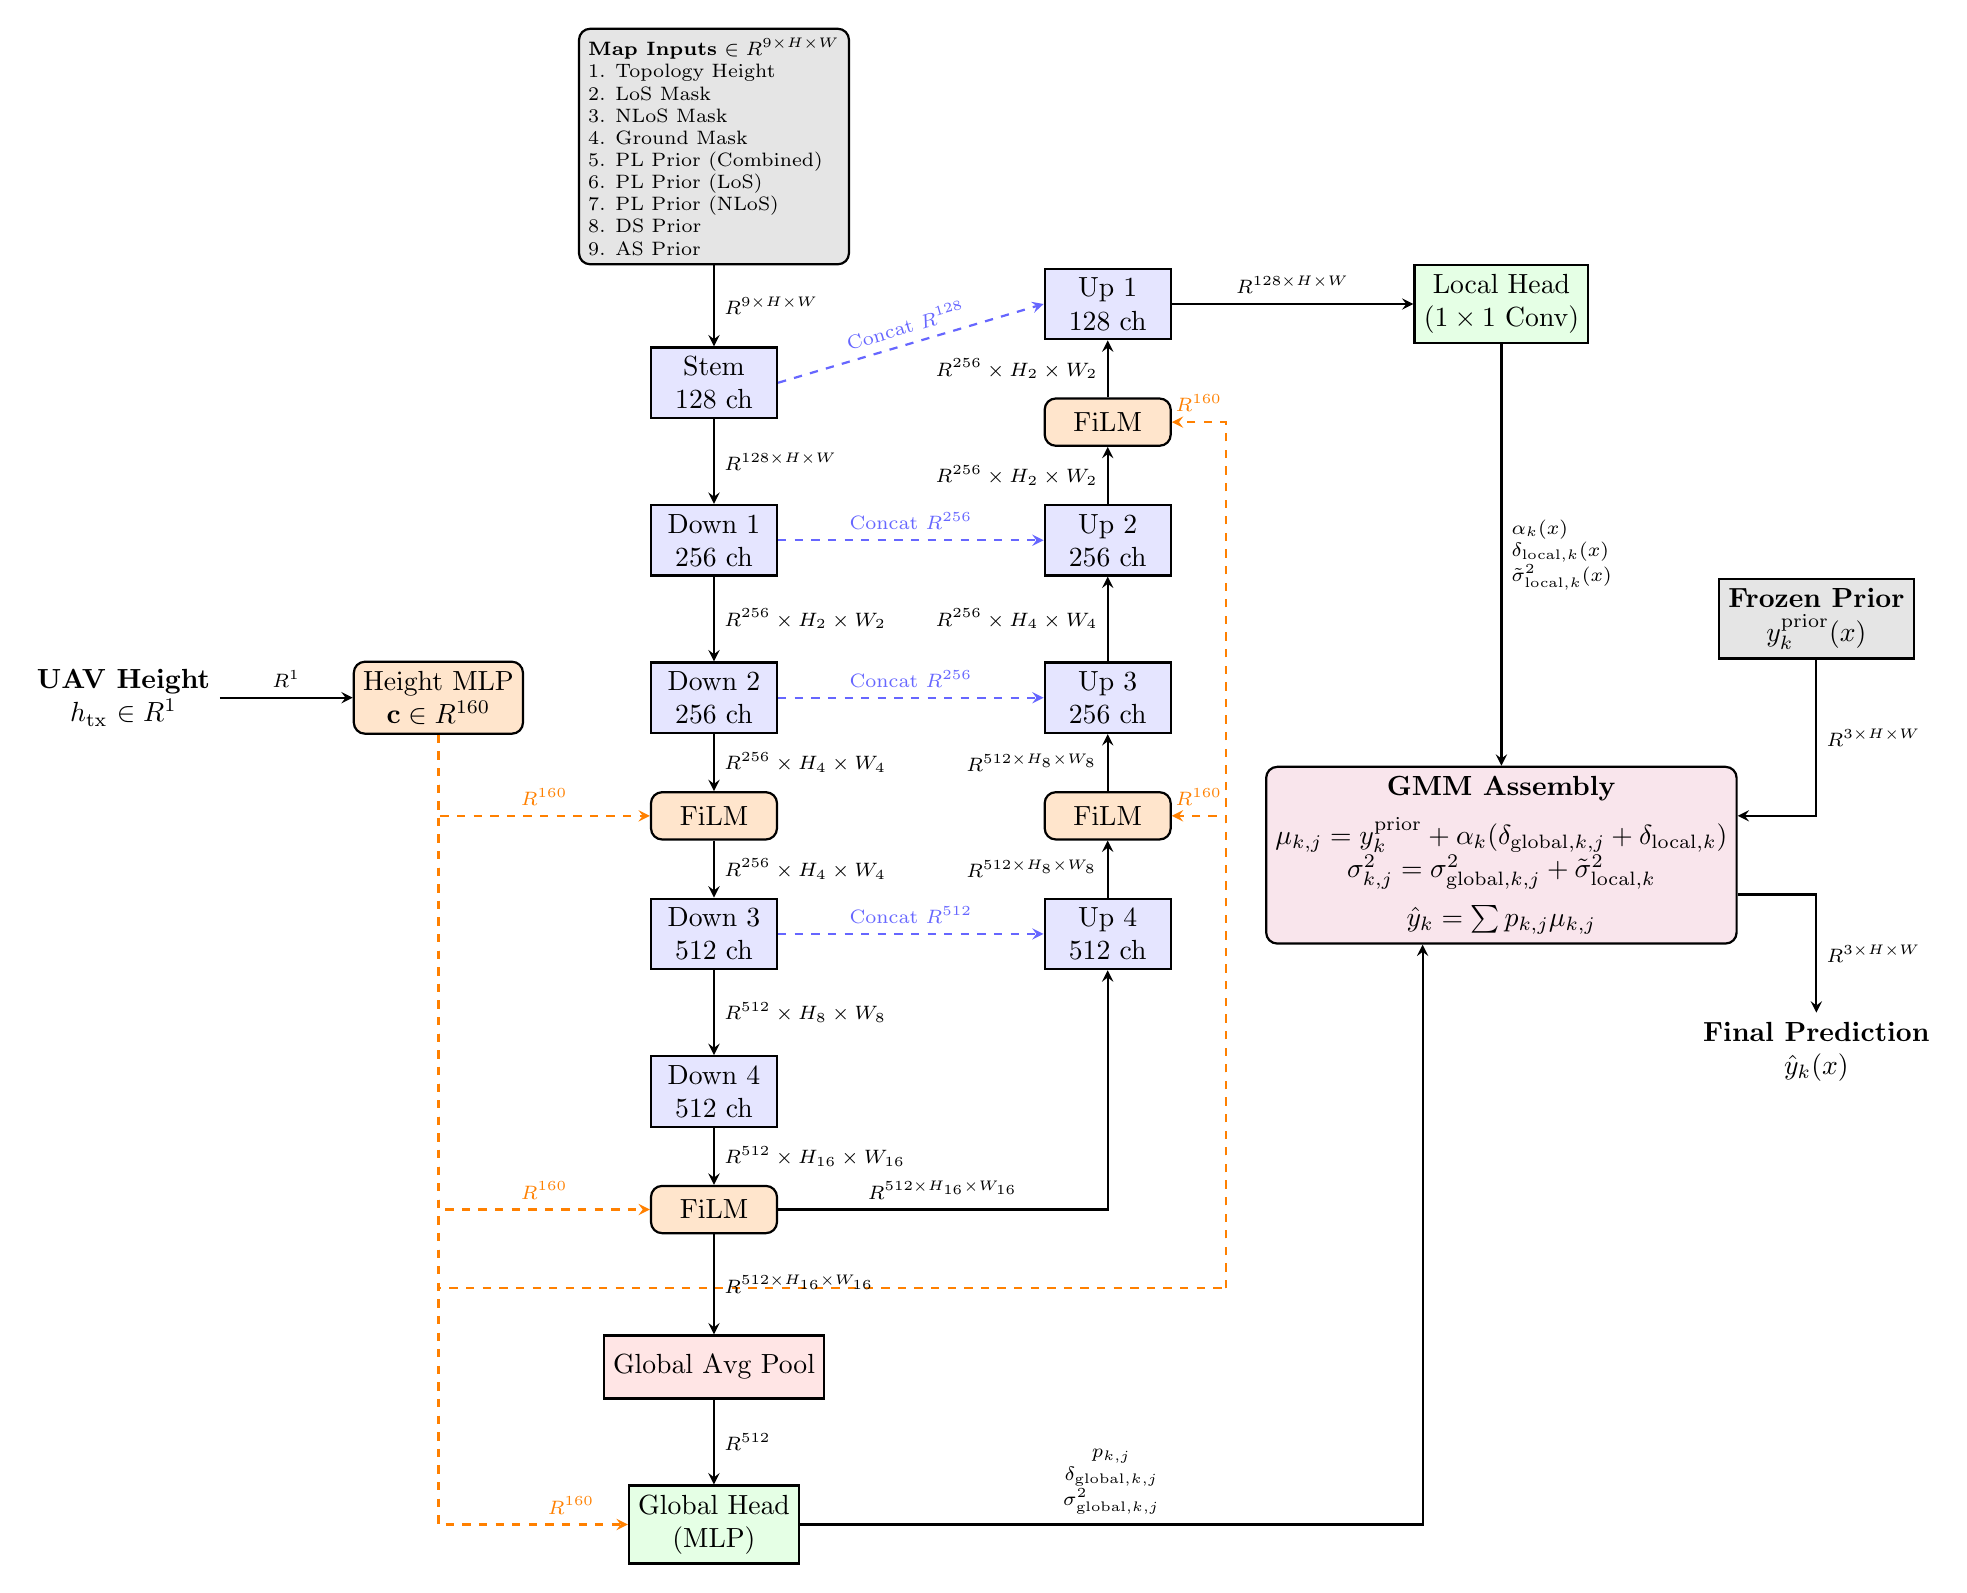
\begin{tikzpicture}[
    >=stealth,
    block/.style={draw, thick, fill=blue!10, rectangle, minimum width=1.6cm, minimum height=0.8cm, align=center},
    pool/.style={draw, thick, fill=red!10, rectangle, minimum width=1.6cm, minimum height=0.8cm, align=center},
    film/.style={draw, thick, fill=orange!20, rectangle, rounded corners, minimum width=1.6cm, minimum height=0.6cm, align=center},
    head/.style={draw, thick, fill=green!10, rectangle, minimum width=2cm, minimum height=0.8cm, align=center},
    gmm/.style={draw, thick, fill=purple!10, rectangle, rounded corners, minimum width=3.5cm, minimum height=2cm, align=center},
    skip/.style={->, thick, blue!60, dashed}
]

% Inputs
\node[align=left, font=\scriptsize, draw, thick, fill=gray!20, rectangle, rounded corners] (in_map) at (0, 3) {\textbf{Map Inputs} $\in \mathbb{R}^{9 \times H \times W}$ \\ 1. Topology Height \\ 2. LoS Mask \\ 3. NLoS Mask \\ 4. Ground Mask \\ 5. PL Prior (Combined) \\ 6. PL Prior (LoS) \\ 7. PL Prior (NLoS) \\ 8. DS Prior \\ 9. AS Prior};
\node[align=center] (in_htx) at (-7.5, -4) {\textbf{UAV Height} \\ $h_{\mathrm{tx}}$ $\in \mathbb{R}^{1}$};

% Height MLP
\node[film] (h_mlp) at (-3.5, -4) {Height MLP \\ $\textbf{c} \in \mathbb{R}^{160}$};
\draw[->, thick] (in_htx) -- node[above, font=\scriptsize] {$\mathbb{R}^{1}$} (h_mlp);

% Encoder (Left Column)
\node[block] (e0) at (0, 0) {Stem \\ 128 ch};
\node[block] (e1) at (0, -2) {Down 1 \\ 256 ch};
\node[block] (e2) at (0, -4) {Down 2 \\ 256 ch};
\node[film] (f2) at (0, -5.5) {FiLM};
\node[block] (e3) at (0, -7) {Down 3 \\ 512 ch};
\node[block] (e4) at (0, -9) {Down 4 \\ 512 ch};
\node[film] (f4) at (0, -10.5) {FiLM};

\draw[->, thick] (in_map) -- node[right, font=\scriptsize] {$\mathbb{R}^{9 \times H \times W}$} (e0);
\draw[->, thick] (e0) -- node[right, font=\scriptsize] {$\mathbb{R}^{128 \times H \times W}$} (e1);
\draw[->, thick] (e1) -- node[right, font=\scriptsize] {$\mathbb{R}^{256} \times H_2 \times W_2$} (e2);
\draw[->, thick] (e2) -- node[right, font=\scriptsize] {$\mathbb{R}^{256} \times H_4 \times W_4$} (f2);
\draw[->, thick] (f2) -- node[right, font=\scriptsize] {$\mathbb{R}^{256} \times H_4 \times W_4$} (e3);
\draw[->, thick] (e3) -- node[right, font=\scriptsize] {$\mathbb{R}^{512} \times H_8 \times W_8$} (e4);
\draw[->, thick] (e4) -- node[right, font=\scriptsize] {$\mathbb{R}^{512} \times H_{16} \times W_{16}$} (f4);

% Decoder (Right Column)
\node[block] (d3) at (5, -7) {Up 4 \\ 512 ch};
\node[film] (fd3) at (5, -5.5) {FiLM};
\node[block] (d2) at (5, -4) {Up 3 \\ 256 ch};
\node[block] (d1) at (5, -2) {Up 2 \\ 256 ch};
\node[film] (fd1) at (5, -0.5) {FiLM};
\node[block] (d0) at (5, 1) {Up 1 \\ 128 ch};

\draw[->, thick] (f4.east) -- node[above, font=\scriptsize] {$\mathbb{R}^{512 \times H_{16} \times W_{16}}$} (5, -10.5) -- (d3.south);
\draw[->, thick] (d3) -- node[left, font=\scriptsize] {$\mathbb{R}^{512 \times H_8 \times W_8}$} (fd3);
\draw[->, thick] (fd3) -- node[left, font=\scriptsize] {$\mathbb{R}^{512 \times H_8 \times W_8}$} (d2);
\draw[->, thick] (d2) -- node[left, font=\scriptsize] {$\mathbb{R}^{256} \times H_4 \times W_4$} (d1);
\draw[->, thick] (d1) -- node[left, font=\scriptsize] {$\mathbb{R}^{256} \times H_2 \times W_2$} (fd1);
\draw[->, thick] (fd1) -- node[left, font=\scriptsize] {$\mathbb{R}^{256} \times H_2 \times W_2$} (d0);

% Skip connections
\draw[skip] (e3.east) -- node[above, font=\scriptsize] {Concat $\mathbb{R}^{512}$} (d3.west);
\draw[skip] (e2.east) -- node[above, font=\scriptsize] {Concat $\mathbb{R}^{256}$} (d2.west);
\draw[skip] (e1.east) -- node[above, font=\scriptsize] {Concat $\mathbb{R}^{256}$} (d1.west);
\draw[skip] (e0.east) -- node[above, sloped, font=\scriptsize] {Concat $\mathbb{R}^{128}$} (d0.west);

% FiLM routing bus (Encoder)
\draw[->, thick, orange, dashed] (h_mlp.south) |- node[pos=0.75, above, font=\scriptsize] {$\mathbb{R}^{160}$} (f2.west);
\draw[->, thick, orange, dashed] (h_mlp.south) |- node[pos=0.75, above, font=\scriptsize] {$\mathbb{R}^{160}$} (f4.west);

% FiLM routing bus (Decoder)
\draw[thick, orange, dashed] (h_mlp.south) |- (6.5, -11.5);
\draw[->, thick, orange, dashed] (6.5, -11.5) |- node[pos=0.75, above, font=\scriptsize] {$\mathbb{R}^{160}$} (fd3.east);
\draw[->, thick, orange, dashed] (6.5, -11.5) |- node[pos=0.75, above, font=\scriptsize] {$\mathbb{R}^{160}$} (fd1.east);

% Global Head Branch
\node[pool] (pool) at (0, -12.5) {Global Avg Pool};
\node[head] (global_head) at (0, -14.5) {Global Head \\ (MLP)};
\draw[->, thick] (f4.south) -- node[right, font=\scriptsize] {$\mathbb{R}^{512 \times H_{16} \times W_{16}}$} (pool.north);
\draw[->, thick] (pool.south) -- node[right, font=\scriptsize] {$\mathbb{R}^{512}$} (global_head.north);
\draw[->, thick, orange, dashed] (h_mlp.south) |- node[pos=0.85, above, font=\scriptsize] {$\mathbb{R}^{160}$} (global_head.west);

% Local Head Branch
\node[head] (local_head) at (10, 1) {Local Head \\ ($1\times1$ Conv)};
\draw[->, thick] (d0.east) -- node[above, font=\scriptsize] {$\mathbb{R}^{128 \times H \times W}$} (local_head.west);

% Prior Input
\node[align=center, draw, thick, fill=gray!20, rectangle, minimum height=0.8cm] (prior) at (14, -3) {\textbf{Frozen Prior} \\ $y_k^{\mathrm{prior}}(x)$};

% GMM Assembly
\node[gmm] (gmm) at (10, -6) {\textbf{GMM Assembly} \\[0.2cm] 
$\mu_{k,j} = y_k^{\mathrm{prior}} + \alpha_k (\delta_{\mathrm{global},k,j} + \delta_{\mathrm{local},k})$ \\ 
$\sigma^2_{k,j} = \sigma_{\mathrm{global},k,j}^2 + \tilde\sigma_{\mathrm{local},k}^2$ \\[0.2cm] 
$\hat y_k = \sum p_{k,j} \mu_{k,j}$};

% Routing Prior to GMM
\draw[->, thick] (prior.south) |- node[pos=0.25, right, font=\scriptsize] {$\mathbb{R}^{3 \times H \times W}$} ([yshift=0.5cm]gmm.east);

% Pixel Level outputs flowing to GMM
\draw[->, thick] (local_head.south) -- node[right, align=left, font=\scriptsize] {$\alpha_k(x)$ \\ $\delta_{\mathrm{local},k}(x)$ \\ $\tilde\sigma_{\mathrm{local},k}^2(x)$} (gmm.north);

% Map Level outputs flowing to GMM
\draw[->, thick] (global_head.east) -| node[pos=0.25, above, align=center, font=\scriptsize] {$p_{k,j}$ \\ $\delta_{\mathrm{global},k,j}$ \\ $\sigma_{\mathrm{global},k,j}^2$} ([xshift=-1cm]gmm.south);

% Final Output
\node[align=center] (final_out) at (14, -8.5) {\textbf{Final Prediction} \\ $\hat y_k(x)$};
\draw[->, thick] ([yshift=-0.5cm]gmm.east) -| node[pos=0.75, right, font=\scriptsize] {$\mathbb{R}^{3 \times H \times W}$} (final_out.north);

\end{tikzpicture}
}
\caption{Schematic of the final huge shared UNet architecture with FiLM conditioning.}
\label{fig:try80_arch}
\end{figure}

\paragraph{Detailed sinusoidal height embedding and FiLM path.}
The scalar UAV height $h_{\mathrm{tx}}$ is first
converted into a 32-dimensional sinusoidal embedding:
\begin{equation}
f_i
=
\exp\!\left(
\log 12
+
\frac{i-1}{15}\bigl(\log 478 - \log 12\bigr)
\right),
\qquad i=1,\dots,16
\end{equation}
\begin{equation}
\textbf{e}(h_{\mathrm{tx}})
=
\left[
\sin\!\left(\frac{h_{\mathrm{tx}}}{f_1}\right), \dots,
\sin\!\left(\frac{h_{\mathrm{tx}}}{f_{16}}\right),
\cos\!\left(\frac{h_{\mathrm{tx}}}{f_1}\right), \dots,
\cos\!\left(\frac{h_{\mathrm{tx}}}{f_{16}}\right)
\right]
\in \mathbb{R}^{32}
\label{eq:try80_height_embed}
\end{equation}

\begin{figure}[H]
\centering
\resizebox{\textwidth}{!}{%
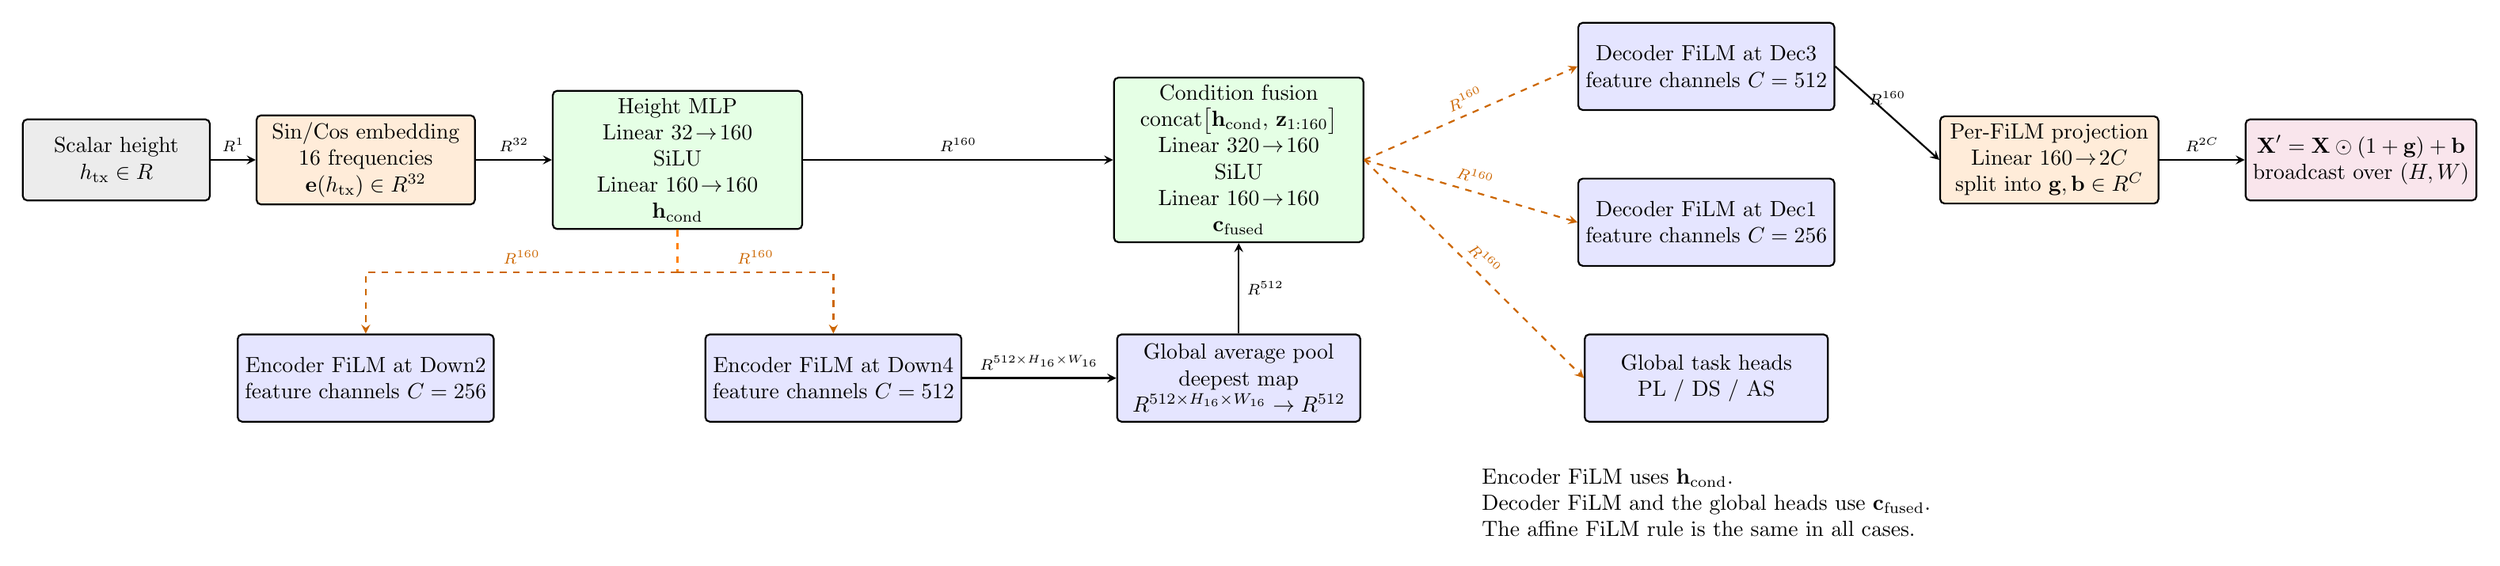
\begin{tikzpicture}[
    >=stealth,
    font=\normalsize,
    smallbox/.style={draw, thick, rounded corners=2pt, rectangle, minimum width=3.0cm, minimum height=1.3cm, align=center},
    opbox/.style={draw, thick, rounded corners=2pt, rectangle, minimum width=3.5cm, minimum height=1.4cm, align=center, fill=orange!15},
    featbox/.style={draw, thick, rounded corners=2pt, rectangle, minimum width=3.9cm, minimum height=1.4cm, align=center, fill=blue!10},
    condbox/.style={draw, thick, rounded corners=2pt, rectangle, minimum width=4.0cm, minimum height=1.4cm, align=center, fill=green!10},
    note/.style={font=\normalsize, align=left},
    arr/.style={->, thick},
    condarr/.style={->, thick, orange!80!black, dashed}
]

\node[smallbox, fill=gray!15] (h) at (0,0) {Scalar height\\$h_{\mathrm{tx}} \in \mathbb{R}$};
\node[opbox] (embed) at (4.0,0) {Sin/Cos embedding\\16 frequencies\\$\textbf{e}(h_{\mathrm{tx}})\in\mathbb{R}^{32}$};
\node[condbox] (mlp1) at (9.0,0) {Height MLP\\Linear $32\!\to\!160$\\SiLU\\Linear $160\!\to\!160$\\$\textbf{h}_{\mathrm{cond}}$};

\draw[arr] (h) -- node[above, font=\scriptsize] {$\mathbb{R}^{1}$} (embed);
\draw[arr] (embed) -- node[above, font=\scriptsize] {$\mathbb{R}^{32}$} (mlp1);

\node[featbox] (enc2) at (4.0,-3.5) {Encoder FiLM at Down2\\feature channels $C=256$};
\node[featbox] (enc4) at (11.5,-3.5) {Encoder FiLM at Down4\\feature channels $C=512$};
\draw[thick, orange, dashed] (mlp1.south) -- (9.0, -1.8);
\draw[condarr] (9.0, -1.8) -- node[above, font=\scriptsize] {$\mathbb{R}^{160}$} (4.0, -1.8) -- (enc2.north);
\draw[condarr] (9.0, -1.8) -- node[above, font=\scriptsize] {$\mathbb{R}^{160}$} (11.5, -1.8) -- (enc4.north);

\node[featbox] (pool) at (18.0,-3.5) {Global average pool\\deepest map\\$\mathbb{R}^{512\times H_{16}\times W_{16}} \to \mathbb{R}^{512}$};
\draw[arr] (enc4.east) -- node[above, font=\scriptsize] {$\mathbb{R}^{512\times H_{16}\times W_{16}}$} (pool.west);

\node[condbox] (fuse) at (18.0,0) {Condition fusion\\concat$\bigl[\textbf{h}_{\mathrm{cond}},\,\textbf{z}_{1:160}\bigr]$\\Linear $320\!\to\!160$\\SiLU\\Linear $160\!\to\!160$\\$\textbf{c}_{\mathrm{fused}}$};
\draw[arr] (mlp1.east) -- node[above, font=\scriptsize] {$\mathbb{R}^{160}$} (fuse.west);
\draw[arr] (pool.north) -- node[right, font=\scriptsize] {$\mathbb{R}^{512}$} (fuse.south);

\node[featbox] (dec3) at (25.5, 1.5) {Decoder FiLM at Dec3\\feature channels $C=512$};
\node[featbox] (dec1) at (25.5,-1.0) {Decoder FiLM at Dec1\\feature channels $C=256$};
\node[featbox] (gh) at (25.5,-3.5) {Global task heads\\PL / DS / AS};
\draw[condarr] (fuse.east) -- node[above, sloped, font=\scriptsize] {$\mathbb{R}^{160}$} (dec3.west);
\draw[condarr] (fuse.east) -- node[above, sloped, font=\scriptsize] {$\mathbb{R}^{160}$} (dec1.west);
\draw[condarr] (fuse.east) -- node[above, sloped, font=\scriptsize] {$\mathbb{R}^{160}$} (gh.west);

\node[opbox] (filmproj) at (31.0,0.0) {Per-FiLM projection\\Linear $160\!\to\!2C$\\split into $\textbf{g},\textbf{b} \in \mathbb{R}^{C}$};
\node[smallbox, fill=purple!10] (affine) at (36.0,0.0) {$\textbf{X}'=\textbf{X}\odot(1+\textbf{g})+\textbf{b}$\\broadcast over $(H,W)$};
\draw[arr] (dec3.east) -- node[above, font=\scriptsize] {$\mathbb{R}^{160}$} (filmproj.west);
\draw[arr] (filmproj.east) -- node[above, font=\scriptsize] {$\mathbb{R}^{2C}$} (affine.west);

\node[note] at (25.5,-5.5) {Encoder FiLM uses $\textbf{h}_{\mathrm{cond}}$.\\Decoder FiLM and the global heads use $\textbf{c}_{\mathrm{fused}}$.\\The affine FiLM rule is the same in all cases.};

\end{tikzpicture}%
}
\caption{Detailed sinusoidal height-conditioning path.}
\label{fig:try80_film_detail}
\end{figure}

\paragraph{Detailed prior-anchored GMM head.}
For each task
$k$ and for each region
$r \in \{\mathrm{LoS},\mathrm{NLoS}\}$, the model predicts a 3-component
mixture. The global head outputs
$\pi^{(g)}_{k,r,j}$, $\delta^{(g)}_{k,r,j}$ and $\sigma^{(g)}_{k,r,j}$, while
the local head outputs per-pixel maps
$p^{(\ell)}_{k,r,j}(x)$, $\delta^{(\ell)}_{k,r}(x)$, $\alpha_{k,r}(x)$, and
$\tilde\sigma_{k,r}(x)$.

\begin{figure}[H]
\centering
\resizebox{\textwidth}{!}{%
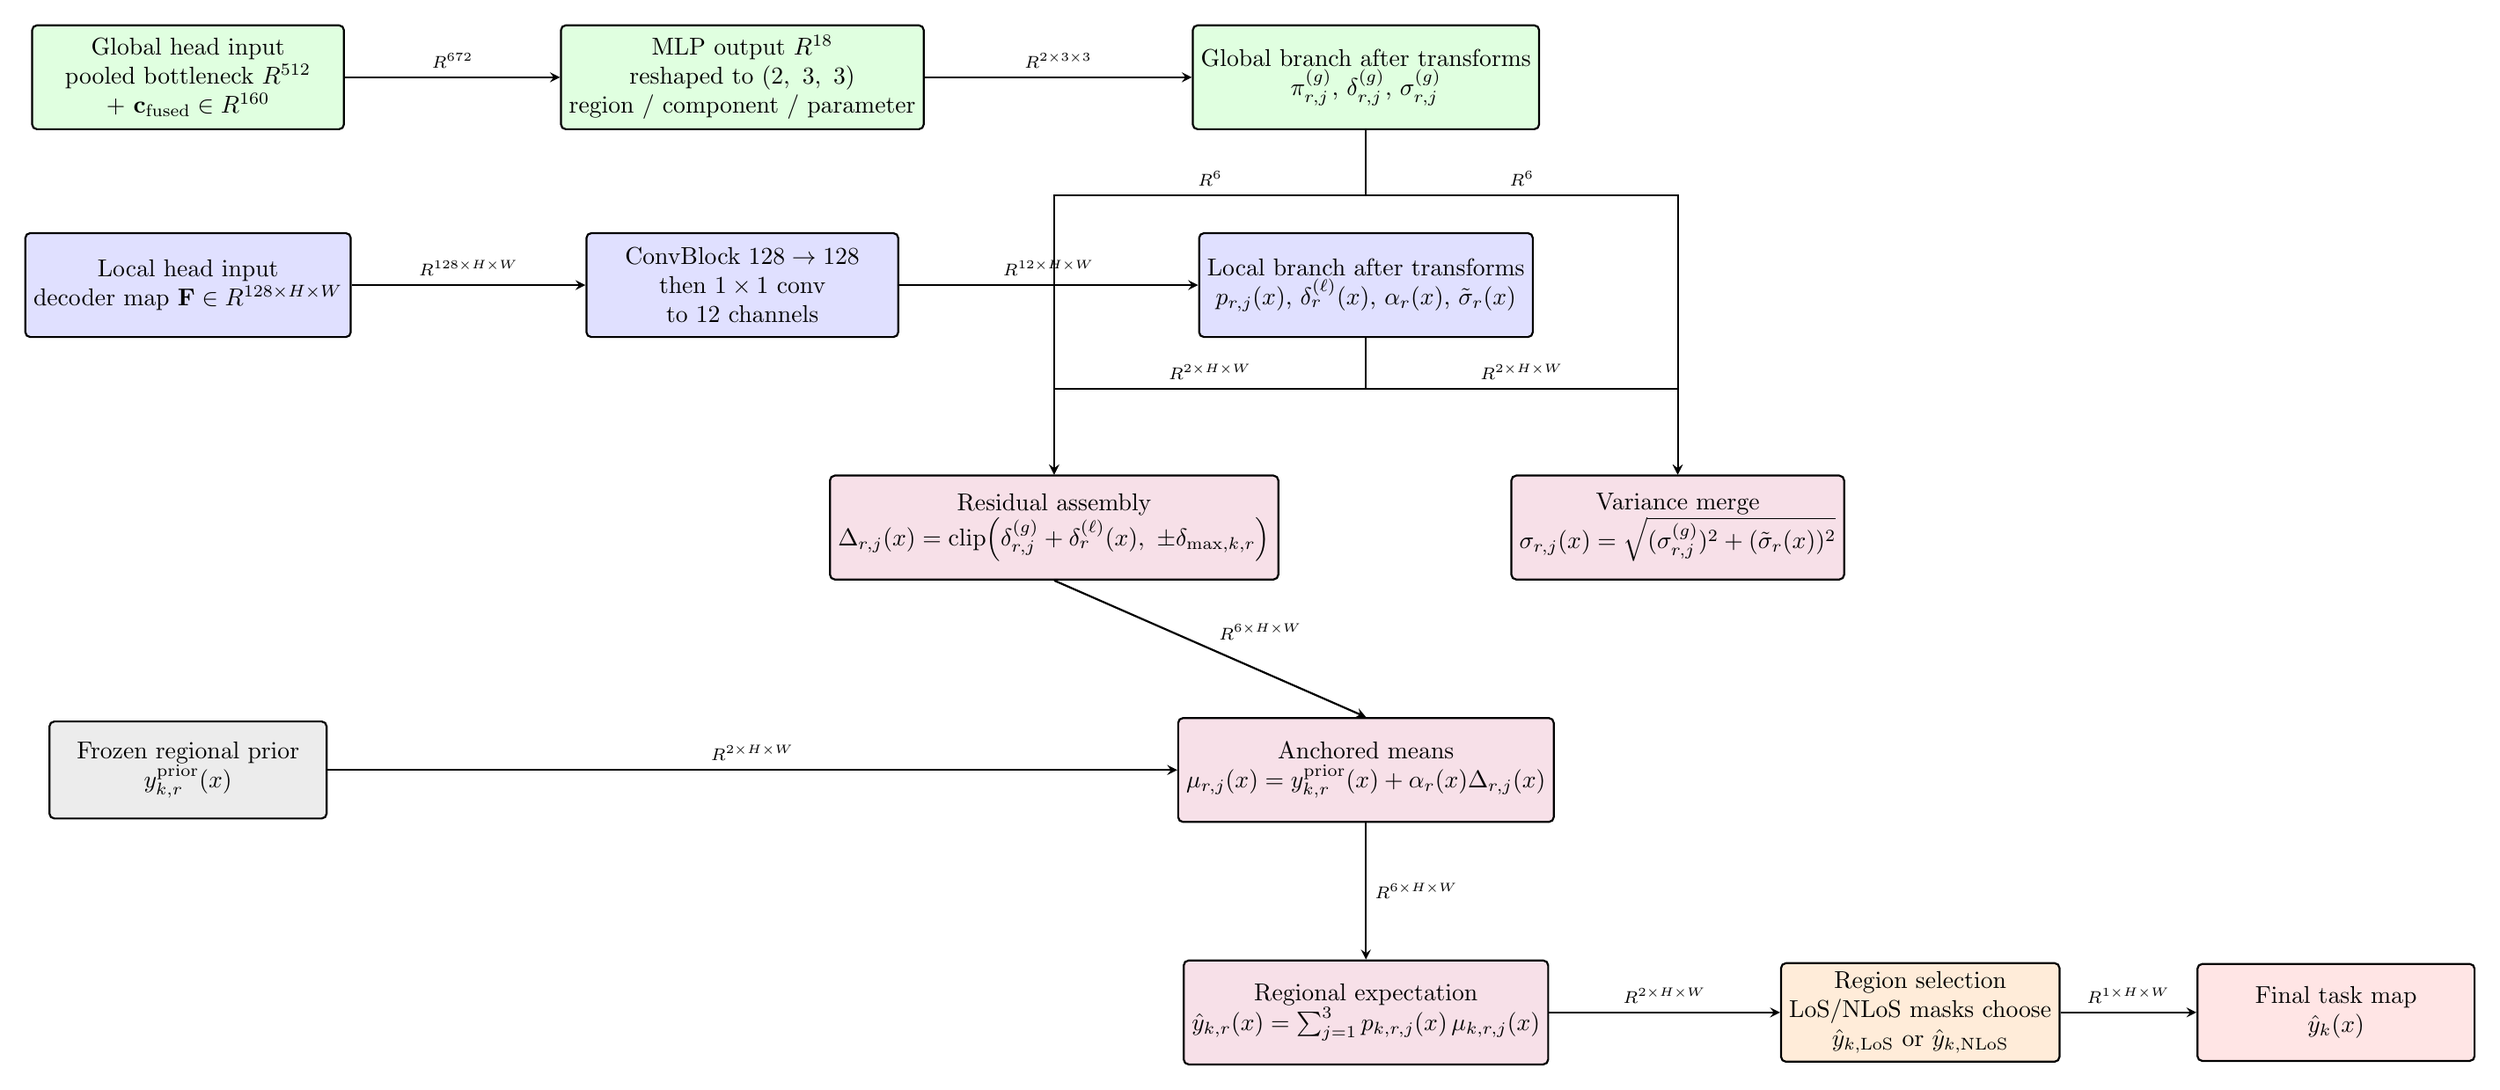
\begin{tikzpicture}[
    >=stealth,
    font=\normalsize,
    box/.style={draw, thick, rounded corners=2pt, rectangle, minimum width=4.0cm, minimum height=1.4cm, align=center},
    prior/.style={draw, thick, rounded corners=2pt, rectangle, minimum width=4.0cm, minimum height=1.4cm, align=center, fill=gray!15},
    global/.style={draw, thick, rounded corners=2pt, rectangle, minimum width=4.5cm, minimum height=1.5cm, align=center, fill=green!12},
    local/.style={draw, thick, rounded corners=2pt, rectangle, minimum width=4.5cm, minimum height=1.5cm, align=center, fill=blue!12},
    mix/.style={draw, thick, rounded corners=2pt, rectangle, minimum width=4.8cm, minimum height=1.5cm, align=center, fill=purple!12},
    arr/.style={->, thick}
]

\node[global] (globin) at (0,3.5) {Global head input\\pooled bottleneck $\mathbb{R}^{512}$\\$+\ \textbf{c}_{\mathrm{fused}}\in\mathbb{R}^{160}$};
\node[global] (globraw) at (8.0,3.5) {MLP output $\mathbb{R}^{18}$\\reshaped to $(2,\ 3,\ 3)$\\region / component / parameter};
\node[global] (globpars) at (17.0,3.5) {Global branch after transforms\\$\pi^{(g)}_{r,j}$, $\delta^{(g)}_{r,j}$, $\sigma^{(g)}_{r,j}$};
\draw[arr] (globin) -- node[above, font=\scriptsize] {$\mathbb{R}^{672}$} (globraw);
\draw[arr] (globraw) -- node[above, font=\scriptsize] {$\mathbb{R}^{2 \times 3 \times 3}$} (globpars);

\node[local] (locin) at (0,0.5) {Local head input\\decoder map $\textbf{F}\in\mathbb{R}^{128\times H \times W}$};
\node[local] (locraw) at (8.0,0.5) {ConvBlock $128\to128$\\then $1\times1$ conv\\to 12 channels};
\node[local] (locpars) at (17.0,0.5) {Local branch after transforms\\$p_{r,j}(x)$, $\delta^{(\ell)}_{r}(x)$, $\alpha_r(x)$, $\tilde\sigma_r(x)$};
\draw[arr] (locin) -- node[above, font=\scriptsize] {$\mathbb{R}^{128 \times H \times W}$} (locraw);
\draw[arr] (locraw) -- node[above, font=\scriptsize] {$\mathbb{R}^{12 \times H \times W}$} (locpars);

\node[mix] (delta) at (12.5,-3.0) {Residual assembly\\$\Delta_{r,j}(x)=\mathrm{clip}\!\left(\delta^{(g)}_{r,j}+\delta^{(\ell)}_{r}(x),\ \pm\delta_{\max,k,r}\right)$};
\node[prior] (prior) at (0,-6.5) {Frozen regional prior\\$y^{\mathrm{prior}}_{k,r}(x)$};
\node[mix] (mu) at (17.0,-6.5) {Anchored means\\$\mu_{r,j}(x)=y^{\mathrm{prior}}_{k,r}(x)+\alpha_r(x)\Delta_{r,j}(x)$};
\node[mix] (sigma) at (21.5,-3.0) {Variance merge\\$\sigma_{r,j}(x)=\sqrt{(\sigma^{(g)}_{r,j})^2+(\tilde\sigma_r(x))^2}$};

\draw[thick] (globpars.south) -- (17.0, 1.8);
\draw[arr] (17.0, 1.8) -- node[above, font=\scriptsize] {$\mathbb{R}^{6}$} (12.5, 1.8) -- (delta.north);
\draw[arr] (17.0, 1.8) -- node[above, font=\scriptsize] {$\mathbb{R}^{6}$} (21.5, 1.8) -- (sigma.north);

\draw[thick] (locpars.south) -- (17.0, -1.0);
\draw[arr] (17.0, -1.0) -- node[above, font=\scriptsize] {$\mathbb{R}^{2 \times H \times W}$} (12.5, -1.0) -- (delta.north);
\draw[arr] (17.0, -1.0) -- node[above, font=\scriptsize] {$\mathbb{R}^{2 \times H \times W}$} (21.5, -1.0) -- (sigma.north);

\draw[arr] (delta.south) -- node[above right, font=\scriptsize] {$\mathbb{R}^{6 \times H \times W}$} (mu.north);
\draw[arr] (prior.east) -- node[above, font=\scriptsize] {$\mathbb{R}^{2 \times H \times W}$} (mu.west);

\node[mix] (expv) at (17.0,-10.0) {Regional expectation\\$\hat y_{k,r}(x)=\sum_{j=1}^{3} p_{k,r,j}(x)\,\mu_{k,r,j}(x)$};
\node[box, fill=orange!15] (mask) at (25.0,-10.0) {Region selection\\LoS/NLoS masks choose\\$\hat y_{k,\mathrm{LoS}}$ or $\hat y_{k,\mathrm{NLoS}}$};
\node[box, fill=red!10] (out) at (31.0,-10.0) {Final task map\\$\hat y_k(x)$};

\draw[arr] (mu.south) -- node[right, font=\scriptsize] {$\mathbb{R}^{6 \times H \times W}$} (expv.north);
\draw[arr] (expv.east) -- node[above, font=\scriptsize] {$\mathbb{R}^{2 \times H \times W}$} (mask.west);
\draw[arr] (mask.east) -- node[above, font=\scriptsize] {$\mathbb{R}^{1 \times H \times W}$} (out.west);

\end{tikzpicture}%
}
\caption{Detailed prior-anchored GMM head used by the final model.}
\label{fig:try80_gmm_detail}
\end{figure}

\subsection{Composite Optimization Objective}
\label{sec:try80_objective}
\begingroup
\setlength{\abovedisplayskip}{5pt plus 1pt minus 1pt}
\setlength{\belowdisplayskip}{5pt plus 1pt minus 1pt}
\setlength{\abovedisplayshortskip}{3pt plus 1pt minus 1pt}
\setlength{\belowdisplayshortskip}{3pt plus 1pt minus 1pt}

The implementation defines a composite loss that can train both the
probabilistic GMM head and the deterministic residual map. For each task, let
\(\Omega_k\) be the valid ground-pixel set, let \(q_k(y\mid x)\) be the
predicted mixture density, and let \(\hat y_k(x)\) be the native-space point
prediction used for RMSE. The total objective is:

\begin{equation}
\begin{aligned}
\mathcal{L}
=
\sum_{k\in\{\mathrm{PL},\mathrm{DS},\mathrm{AS}\}}
w_k
\Bigl[
&\lambda_{\mathrm{NLL}}\mathcal{L}_{\mathrm{NLL},k}
+
\lambda_{\mathrm{KL}}\mathcal{L}_{\mathrm{KL},k}
+
\lambda_{\mathrm{mom}}\mathcal{L}_{\mathrm{mom},k}
\\
&+
\lambda_{\mathrm{anchor}}\mathcal{L}_{\mathrm{anchor},k}
+
\lambda_{\mathrm{guard}}\mathcal{L}_{\mathrm{guard},k}
+
\lambda_{\mathrm{out}}\mathcal{L}_{\mathrm{out},k}
\\
&+
\lambda_{\mathrm{RMSE}}\mathcal{L}_{\mathrm{RMSE},k}
+
\lambda_{\mathrm{MAE}}\mathcal{L}_{\mathrm{MAE},k}
\Bigr].
\end{aligned}
\label{eq:try80_total_loss}
\end{equation}

Table~\ref{tab:try80_loss_settings} gives the resolved weights for both the
huge relaxed-residual stage and the final path-loss fine-tune; the equations
below define the terms used in that table.

\paragraph{Map negative log-likelihood.}
The likelihood is computed separately in LoS and NLoS regions, then averaged
over the non-empty regions. For a transformed target \(z_k(x)\),
\begin{equation}
q_{k,r}\!\left(z_k(x)\mid x\right)
=
\sum_{j=1}^{3}
p_{k,r,j}(x)
\mathcal{N}
\left(
z_k(x);
\mu_{k,r,j}(x),
\sigma^2_{k,r,j}(x)
\right),
\label{eq:try80_mixture_density}
\end{equation}
and the regional NLL is
\begin{equation}
\mathcal{L}_{\mathrm{NLL},k,r}
=
-
\frac{1}{|\Omega_{k,r}|}
\sum_{x\in\Omega_{k,r}}
\log q_{k,r}\!\left(z_k(x)\mid x\right).
\label{eq:try80_nll}
\end{equation}
The implemented version evaluates Eq.~\eqref{eq:try80_nll} using
\(\log\sum\exp\) for numerical stability.

\paragraph{Distributional KL term.}
The global branch predicts residual components
\(\delta^{(g)}_{k,r,j}\). To keep those components aligned with the empirical
residual distribution of the current batch, residuals
\(\epsilon_k(x)=y_k(x)-y^{\mathrm{prior}}_k(x)\) are softly binned into an
empirical probability vector \(\textbf{u}_{k,r}\). The global mixture offsets
define a predicted residual histogram \(\textbf{v}_{k,r}\). The loss is
\begin{equation}
\mathcal{L}_{\mathrm{KL},k}
=
\frac{1}{2}
\sum_{r\in\{\mathrm{LoS},\mathrm{NLoS}\}}
\sum_{b=1}^{B}
u_{k,r,b}
\log
\frac{u_{k,r,b}}{v_{k,r,b}},
\qquad B=64.
\label{eq:try80_kl}
\end{equation}
This term does not force a perfect pixel-wise correction. It only encourages
the map-level mixture to place probability mass where the batch residuals
actually live.

\paragraph{Moment matching.}
The point prediction is also constrained to have approximately the same first
two moments as the target map:
\begin{equation}
\mathcal{L}_{\mathrm{mom},k}
=
\left(\bar{\hat y}_k-\bar y_k\right)^2
+
\left(s_{\hat y,k}-s_{y,k}\right)^2,
\label{eq:try80_moment}
\end{equation}
where bars denote masked means over \(\Omega_k\) and \(s\) denotes masked
standard deviation. When active, this term prevents a low-NLL solution from
matching local density while drifting in map-average level. In the final
fine-tune it is defined by the code but has zero weight.

\paragraph{Anchor and guard terms.}
The anchor penalty keeps the correction small:
\begin{equation}
\mathcal{L}_{\mathrm{anchor},k}
=
\mathbb{E}
\left[
\alpha_k(x)^2
+
0.25\left(\delta^{(g)}_k\right)^2
+
0.50\left(\delta^{(\ell)}_k(x)\right)^2
\right].
\label{eq:try80_anchor}
\end{equation}
The guard term is Eq.~\eqref{eq:try80_loss}. Together, these two terms encode
the final design philosophy: the DNN is allowed to improve the
prior, but it must pay a penalty for large or harmful deviations.

\paragraph{Outlier budget and deterministic losses.}
The last mixture component is treated as the broad/outlier component. If the
outlier-budget term is active and its mean usage exceeds \(\tau=0.60\), a
hinge penalty is applied:
\begin{equation}
\mathcal{L}_{\mathrm{out},k}
=
\max\left(
0,\
\frac{1}{|\Omega_k|}
\sum_{x\in\Omega_k}
p_{k,\mathrm{out}}(x)
-
\tau
\right).
\label{eq:try80_outlier}
\end{equation}
The RMSE and MAE terms are conventional masked deterministic losses:
\begin{equation}
\mathcal{L}_{\mathrm{RMSE},k}
=
\sqrt{
\frac{1}{|\Omega_k|}
\sum_{x\in\Omega_k}
\left(\hat y_k(x)-y_k(x)\right)^2
},
\qquad
\mathcal{L}_{\mathrm{MAE},k}
=
\frac{1}{|\Omega_k|}
\sum_{x\in\Omega_k}
\left|\hat y_k(x)-y_k(x)\right|.
\label{eq:try80_rmse_mae_loss}
\end{equation}

\begin{figure}[H]
\centering
\resizebox{\textwidth}{!}{%
\begin{tikzpicture}[
  >=Stealth,
  box/.style={draw, thick, rounded corners=3pt, align=center,
              minimum height=0.9cm, font=\footnotesize},
  term/.style={box, fill=blue!10, minimum width=2.7cm},
  reg/.style={box, fill=orange!15, minimum width=2.7cm},
  totalbox/.style={box, fill=green!12, minimum width=3.2cm},
  arr/.style={->, thick}
]
\node[term] (nll) at (0,0) {GMM NLL\\pixel density};
\node[term] (kl) at (3.2,0) {KL\\residual histogram};
\node[term] (mom) at (6.4,0) {Moment\\mean/std};
\node[reg] (anchor) at (9.6,0) {Anchor\\small residuals};
\node[reg] (guard) at (12.8,0) {Prior guard\\do no worse};
\node[reg] (outlier) at (16.0,0) {Outlier\\budget};
\node[term] (rmse) at (19.2,0) {RMSE/MAE\\point map};
\node[totalbox] (total) at (9.6,-2.1) {Weighted sum\\$\mathcal{L}$};
\foreach \n in {nll,kl,mom,anchor,guard,outlier,rmse}
  \draw[arr] (\n.south) -- (total.north);
\end{tikzpicture}%
}
\caption[Composite final loss family]{Composite final
loss family. In the final path-loss fine-tuning stage, the selected checkpoint
keeps the GMM head and uses RMSE/MAE, anchor and guard penalties; NLL, KL,
moment and outlier-budget weights are set to zero. Earlier relaxed-residual
runs used non-zero probabilistic weights.}
\label{fig:try80_loss_terms}
\end{figure}
\endgroup
